\chapter{2012}
\label{cha:2012}

\section{Primera parte}
\label{sec:primera-parte}

\begin{Problema}{1}
  El precio de un pastel era de $200$ pesos, pero subi\'o un
  $25\%$. Sobre ese nuevo precio, se puso en oferta. Result\'o que con
  la oferta, el pastel volvi\'o a costar $200$ pesos. ?`De cu\'anto
  fue la oferta?

  \begin{inparaenum}
  \item $23\%$ \esp
  \item $25\%$ \esp
  \item $20\%$ \esp
  \item $35\%$ \esp
  \item De otro porcentaje
  \end{inparaenum}
\end{Problema}

\begin{Solucion}
  
\end{Solucion}

\begin{Problema}{2}
  En un torneo de ping-pong hay ocho jugadores. Si cada uno de ellos
  juega una vez contra cada uno de los otros siete, ?`cu\'antos
  partidos se juegan en total?

  \begin{inparaenum}
  \item $8$ \esp
  \item $56$ \esp
  \item $28$ \esp
  \item $49$ \esp 
  \item Otro n\'umero
  \end{inparaenum}
\end{Problema}

\begin{Solucion}
  
\end{Solucion}

\begin{Problema}{3}
  Considera la sucesi\'on de numeros $1, 3, 7, 13, 21, \cdots\,$ (los
  puntos suspensivos significan que es una lista infinita de
  n\'umeros, por lo que no la podemos escribir toda). El n\'umero que
  aparece en el lugar $n$ lo puedes calcular con la f\'ormula
  $n^2-n+1$ (por ejemplo, el n\'umero que aparece en el quinto lugar
  es $5^2-5+1=21$). ?`Qu\'e n\'umero le sigue al $91$ en la
  sucesi\'on?

  \begin{inparaenum}
  \item El $91$ no est\'a en la sucesi\'on \esp
  \item $98$ \esp
  \item $109$ \esp
  \item $111$ \esp 
  \item Otro n\'umero distinto de los anteriores 
\end{inparaenum}
\end{Problema}

\begin{Solucion}
  
\end{Solucion}

\begin{Problema}{4}
  Tres tristes tigres tragaban trigo en treinta tristes trastos en un
  trigal.  El primer tigre trag\'o el doble de tristes trastos de
  trigo que el segundo tigre, mientras que el segundo tigre trag\'o el
  triple de tristes trastos de trigo que el tercer tigre.  ?`Cu\'antos
  tristes trastos de trigo trag\'o el tercer tigre?

  \begin{inparaenum}
  \item $15$ \esp
  \item $10$ \esp
  \item $5$ \esp
  \item $20$ \esp
  \item Otro n\'umero de trastos
  \end{inparaenum}
\end{Problema}

\begin{Solucion}
  
\end{Solucion}

\begin{Problema}{5}
  Considera un rect\'agulo cuyas longitudes de sus lados son n\'umeros enteros. Si 
  el \'area del rect\'angulo es 21, ?`cu\'ales son los posibles valores de sus lados?

  \begin{inparaenum}
  \item $20$ y $44$ \quad\qquad
  \item $15$ y $30$ \quad\qquad
  \item $17$ y $44$ \quad\qquad
  \item $10$ y $22$ \quad\qquad
  \item Otro par de valores
  \end{inparaenum}
\end{Problema}

\begin{Solucion}
  
\end{Solucion}

\begin{Problema}{6}
  En un c\'irculo se encuentra inscrito un tri\'angulo equil\'atero, como en la figura. 
  Si el \'area del tri\'angulo es uno, ?`cu\'al es el valor del \'area de la regi\'on 
  sombreada?

  \begin{center}
    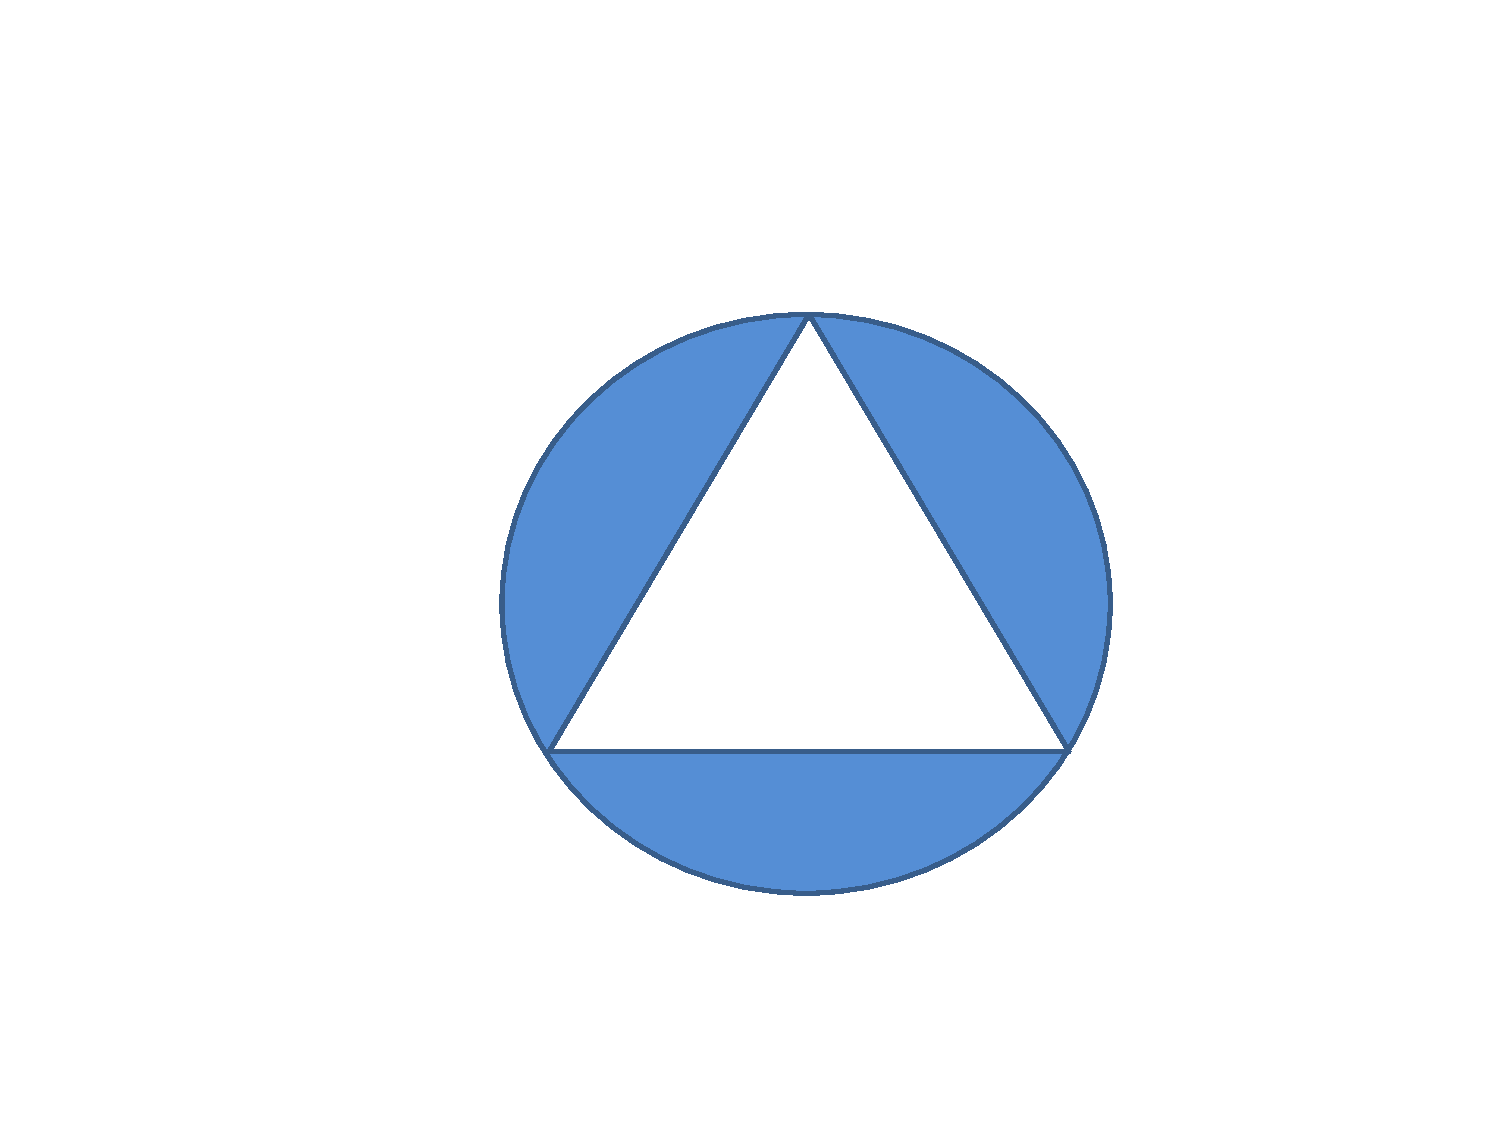
\includegraphics[scale=0.20]{critri.pdf}
  \end{center}

  \begin{inparaenum}
  \item $\dfrac{4\pi}{3\sqrt{3}}-1$, \quad\qquad
  \item $\dfrac{4\pi}{\sqrt{3\sqrt{3}}}-1$ \quad\qquad
  \item $\dfrac{4\pi}{9}-1$ \quad\qquad
  \item $\dfrac{4\pi}{3}-1$ \quad\qquad 
  \item Otro valor
  \end{inparaenum}
\end{Problema}

\begin{Solucion}
  
\end{Solucion}

\begin{Problema}{7}
  El ayuntamiento de Mineral de la Reforma te ha encargado pintar las
  cuatro caras exteriores de un monumento piramidal como el que se
  muestra en la figura. La pir\'amide es lisa, tiene una base cuadrada
  de 16 metros de lado y una altura de 6 metros. Una cubeta de pintura
  cuesta 900 pesos y con ella puedes pintar 40 metros
  cuadrados. ?`Cu\'anto cuesta toda la pintura que necesitas?

  \begin{center}
    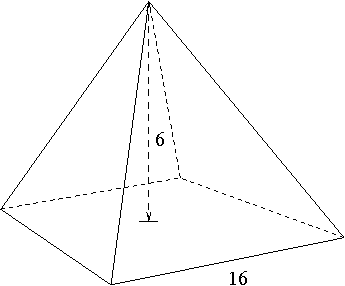
\includegraphics[scale=.44]{OHMpyramid.png}
  \end{center}

  \begin{inparaenum}
  \item $\$7,200$ \quad\qquad
  \item $\$12,960$ \quad\qquad
  \item $\$4,320$ \quad\qquad
  \item $\$10,800$ \quad\qquad
  \item Otra cantidad
  \end{inparaenum}
\end{Problema}

\begin{Solucion}
  
\end{Solucion}

\begin{Problema}{8}
  ?`Cu\'al es el valor m\'as grande que puede tomar la cantidad 
  $\displaystyle{(m+n)/n}$, si sabes que $m$ y $n$ son n\'umeros enteros positivos 
  tales que $n>99$ y $m<101$?

  \begin{inparaenum}
  \item 2 \esp
  \item 7 \esp
  \item 38 \esp
  \item 5 \esp
  \item Ninguno de los valores anteriores
  \end{inparaenum}
\end{Problema}

\begin{Solucion}
  
\end{Solucion}

\begin{Problema}{9}
  En una tina con agua como la de la figura, flota una pelota de $60$
  cent\'imetros de di\'ametro. Si el di\'ametro de la tina es de $180$
  cent\'imetros y exactamente un cuarto del volumen de la pelota se
  encuentra sumergida en la tina, ?`cu\'antos cent\'imetros bajar\'a
  el nivel del agua en el recipiente cuando se saque la pelota? El
  volumen total de la pelota es de $36,000\pi$ cm$^3$.

  \begin{center}
    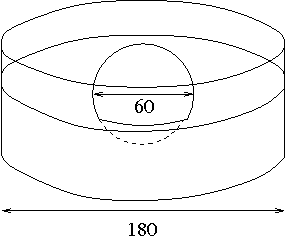
\includegraphics[scale=.58]{OHMballinpool.png}
  \end{center}

  \begin{inparaenum}
  \item $1$ cm\esp
  \item $\dfrac{\pi}{3}$ cm \esp
  \item $\dfrac{10}{9} $ cm\esp
  \item $\dfrac{\pi}{2}$\esp
  \item Otra cantidad
  \end{inparaenum}  
\end{Problema}

\begin{Solucion}
  
\end{Solucion}

\begin{Problema}{10}
  Chaco planea robar un banco y le promete darle al Roto un tercio del
  bot\'in si le ayuda. El Roto acepta, pero como no sabe manejar, le
  pide ayuda al Pepis a cambio de darle un tercio de lo que ganar\'a
  por el robo. El Pepis acepta, pero su auto est\'a en el taller,
  as\'i que le dice al Chueco que si le deja usar su auto, le dar\'a
  un tercio de lo que \'el gane. El Chueco acepta, pero como no oye
  bien, le dice al Pollo que si le ayuda le dar\'a un tercio de lo que
  gane. El Pollo acepta. Tres d\'ias despu\'es del robo atrapan al
  Chueco con su parte del bot\'in, que es de 40,000 pesos.  ?`Cu\'anto
  dinero se llevaron entre todos?

  \begin{inparaenum}
  \item \$810,000 \quad\quad
  \item \$3,240,000 \quad\quad
  \item \$1,620,000 \quad\quad
  \item \$1,000,000 \quad\quad 
  \item Otra cantidad
  \end{inparaenum}
\end{Problema}

\begin{Solucion}
  
\end{Solucion}

\section{Segunda parte}
\label{sec:segunda-parte}

\begin{Problema}{11}
  Paco y Luis se tienen que formar en una fila con sus compa\~neros
  Carlos, Miguel, Daniel y Joel. ?`De cu\'antas formas distintas se
  pueden acomodar de manera que entre Luis y Paco se encuentren
  formados exactamente dos de sus compa\~neros?
\end{Problema}

\begin{Solucion}
  
\end{Solucion}

\begin{Problema}{12}
  Si $c$ es la longitud de la hipotenusa de un tri\'angulo
  rect\'angulo cuyos otros dos lados tienen longitudes $a$ y $b$,
  muestra que $a+b\leq\sqrt{2}c$.
\end{Problema}

\begin{Solucion}
  
\end{Solucion}

\begin{Problema}{13}
  Considera un c\'irculo con centro $O$, como se muestra en la figura.
  $DEB$ es una cuerda del c\'irculo tal que $DE=3$ y $EB=5$. Si $AC$
  es un di\'ametro del c\'irculo que pasa por el punto $E$ y $EC=1$,
  ?`cu\'anto debe medir el radio del c\'irculo?

  \begin{center}
    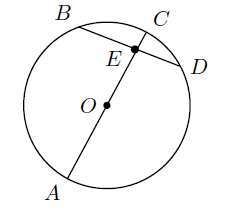
\includegraphics[scale=0.85]{problema2.png}
  \end{center}
\end{Problema}

\begin{Solucion}
  
\end{Solucion}


%%% Local Variables: 
%%% mode: latex
%%% TeX-master: "libro"
%%% End: 